\documentclass[12 pt]{article}
\usepackage[letterpaper]{geometry}
\usepackage{times}
\geometry{top=1.5in, bottom=1.0in, left=1.0in, right=1.0in}

\usepackage[hidelinks]{hyperref}
%\renewcommand{\sectionautorefname}{\S}
\usepackage{xcolor}
\hypersetup{
	colorlinks,
	linkcolor={blue!50!black},
	citecolor={blue!50!black},
	urlcolor={blue!80!black}
}


\usepackage{graphicx} %for images
\graphicspath{{images/}}
\usepackage{caption}
\captionsetup[table]{skip=0pt,singlelinecheck=off}
\captionsetup[figure]{skip=0pt,singlelinecheck=off}
\usepackage{subcaption}


\usepackage{booktabs}
\usepackage{enumitem} %customize list numberings

\usepackage[natbibapa]{apacite}
\usepackage{natbib}

\usepackage{tipa}
\newcommand{\nt}[1]{\textipa{[#1]}} % narrow transcription
\newcommand{\wt}[1]{\textipa{/#1/}} % wide transcription


\usepackage{fancyhdr}
\pagestyle{fancy}
\fancyhf{}
\renewcommand{\headrulewidth}{0pt}
\fancyhead[R]{\thepage}

\usepackage{setspace}
\doublespacing

\usepackage{comment}

\newlength\mystoreparindent
\newenvironment{myparindent}[1]{%
	\setlength{\mystoreparindent}{\the\parindent}
	\setlength{\parindent}{#1}
}{%
	\setlength{\parindent}{\mystoreparindent}
}

\usepackage{easyReview}

%-----------------------------

%-----------------------


\title{Supplementary material: power analysis}
\date{}
%\maketitle

\begin{document}
	\bibliographystyle{apacite}

\section*{Supplementary material: power analysis}

Owing to participant availability given our inclusion criteria, we were able to recruit 10 participants for this study (c.f. section Participants in main article). As part of the peer review process, we carried out post-hoc power analyses using the \textit{mixedpower} package \citep{kumle2021estimating} in R. Although there is a body of literature that debates the usefulness of post-hoc power analyses in interpreting the findings of a completed study where statistical analyses have already been performed \citep{lakens_2021,dziak2020interpretation,lenth2007post,gelman2019observed_effect_size}, we have included this section as a discussion around considerations for power calculation in bilingualism research. 

The aim of the analysis was to explore the power of our experiment design to detect the effects we are investigating. The package simulates responses based on a given dataset and runs the specified analyses on these new data, estimating power by calculating how frequently statistical significance is obtained in the simulated data. The target of the analysis was to calculate the power for detecting an effect for our main variables of interest: vowel*context (to test the hypotheses L2-vowels and Asymmetry), and vowel*context*task (to test the hypothesis Paradigm). 

Power is a function of sample size and effect size. Thus, a key issue in power analyses is to estimate the expected effect size for the treatment/factor of interest \citep{brysbaert2018power, kumle2021estimating}. This may be expressed by a variety of measures, including Cohen's d, $\eta ^2$, and model estimates ($\beta$). Using observed effect sizes from the data for power analyses has been shown to be meaningless \citep{hoenig2001abuse, gelman2019observed_effect_size}, since such ``observed power" is a function of the p-value. Therefore, we need a reasonable estimate of effect size. One way to do this is to use effect sizes reported in other existing literature (however, see \cite{brysbaert2018power} who recommends against using effect sizes from single published studies, as these tend to be inflated), or meta analyses. An alternative approach is to define a smallest effect size that is meaningful to us (smallest effect size of interest; SESOI \citep{kumle2021estimating}), and test whether the study has enough power to detect such an effect, if it were to exist. This value needs to be theoretically motivated. To the best of our knowledge, there is no existing literature on typical effect sizes for spectral differences in cross-language vowel production, and not many studies that report effect sizes. Only more discussion in this field will lead to a consensus on what is considered a typical or minimally meaningful cross-language effect. Similarly, while differences between language-switching paradigms have been informally discussed in previous literature, we are not aware of any study that has measured these differences in a controlled experimental setup, and thus no reported effect sizes for between-paradigm differences in phonetic transfer to act as a guideline. 

Cohen \citeyearpar{cohen1988statistical} classifies effect sizes (Cohen's d values) as small ($\leq$0.2), medium (0.5), and large ($\geq$ 0.8). Although the usefulness of this classification has been debated in the literature, these are often used as ballpark values for power analyses in psychological studies (for a discussion, see \cite{brysbaert2018power}). However, this approach does not generalize well to mixed-effects analyses, particularly for complex models with multiple random effects and interactions, as is typical in psycholinguistic and bilingualism research. ``Determining the SESOI for (G)LMMs is difficult in a simulation-based approach where effect sizes are indicated through the model’s unstandardized beta coefficients...relating effect sizes to beta coefficients in complex models is far from trivial and the authors therefore refrain from making specific recommendations. \citep{kumle2021estimating}". 

The results of a power analysis are only as meaningful as the assumptions that go into it. To avoid making arbitrary assumptions, we followed the approach in \cite{brysbaert2018power} (and discussed in \cite{kumle2021estimating}) of extracting the effect sizes from the study of interest and directly modifying all the beta coefficients by a fixed percentage. Note that we are not assuming that doing so gets us closer to a ``true effect size". Instead, we run simulations with a range of effect sizes and report the power of our study to plausibly detect an effect of that size. The results are shown in the plots in figures \ref{figure_power_analysis_f1} and \ref{figure_power_analysis_f2}. Each panel presents power analysis at a different effect size, and is based on 500 simulations. The plots show power (y-axis) over a range of sample sizes (x-axis), given the assumed effect size.   

As expected, power increases as a function of sample size for all effects. However, of greater interest to us is the differences between the power curves in the four panels (a,b,c,d). These demonstrate how results of the power analysis vary as a function of assumed effect size. Note the the range of effect sizes used here is fairly narrow, varying between 15\% smaller and 15\% greater than the observed effect sizes. These differences demonstrate the importance of theoretically justified effect size estimates before attempting to make inferences based on power analyses. This applies equally to aposteriori power analyses done to make decisions about sample sizes prior to data collection (to reiterate, post-hoc power analyses are best avoided). This emphasizes the importance for bilingualism studies to report effect sizes as a part of their results, which can facilitate discussions and meta-analyses that eventually lead to such norms being established in the field. \footnote{Thanks to the anonymous reviewer at BLC for initiating a fruitful discussion around this.}

\newpage
\begin{figure} \label{figure_power_analysis_f1}
	\centering
	\begin{subfigure}[t]{0.8\textwidth}
		\centering
		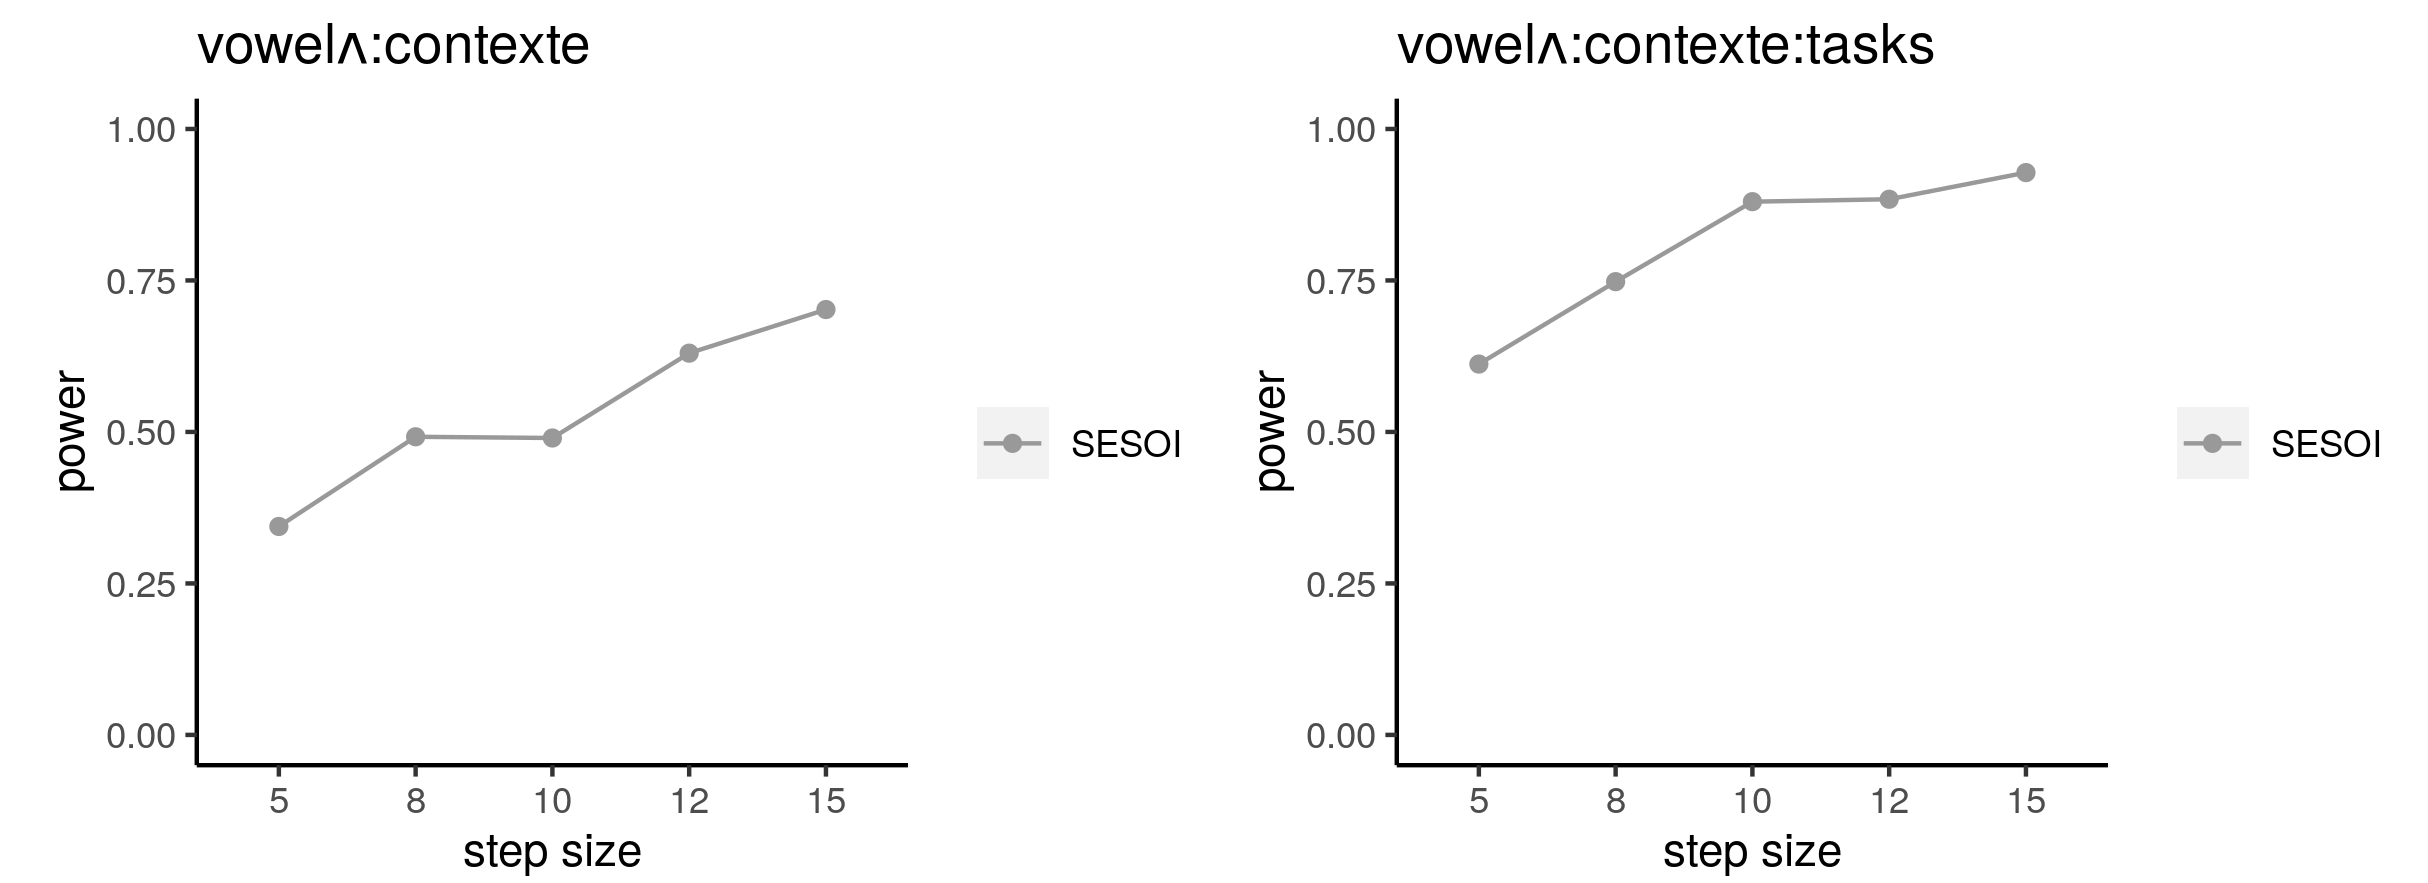
\includegraphics[width=\textwidth]{powerplot_f1_minus15} 
		\caption{Effect size = observed effect size - 15\%} \label{f1_minus15}
	\end{subfigure}
	
	\begin{subfigure}[t]{0.8\textwidth}
		\centering
		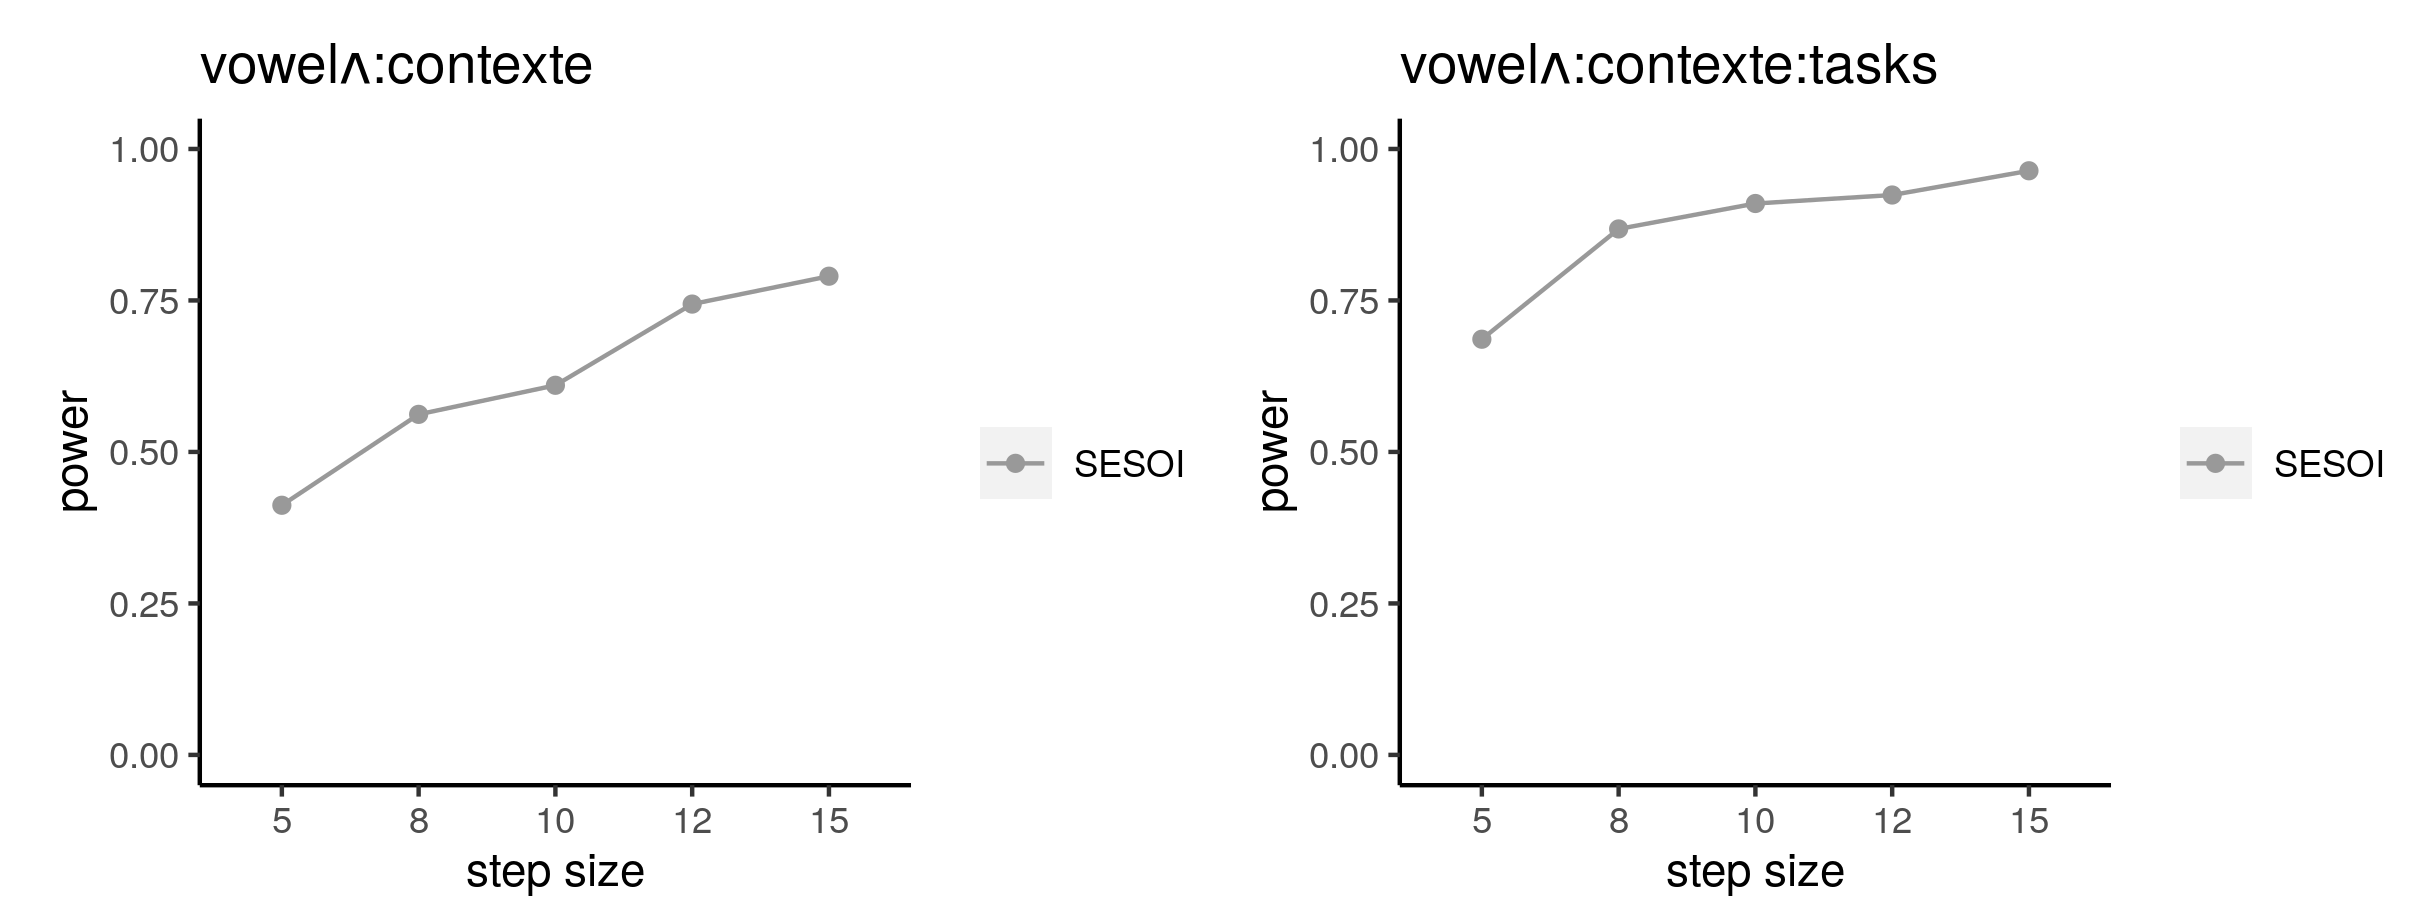
\includegraphics[width=\textwidth]{powerplot_f1_minus5} 
		\caption{Effect size = observed effect size - 5\%} \label{f1_minus5}
	\end{subfigure}
	
	
	\begin{subfigure}[t]{0.8\textwidth}
		\centering
		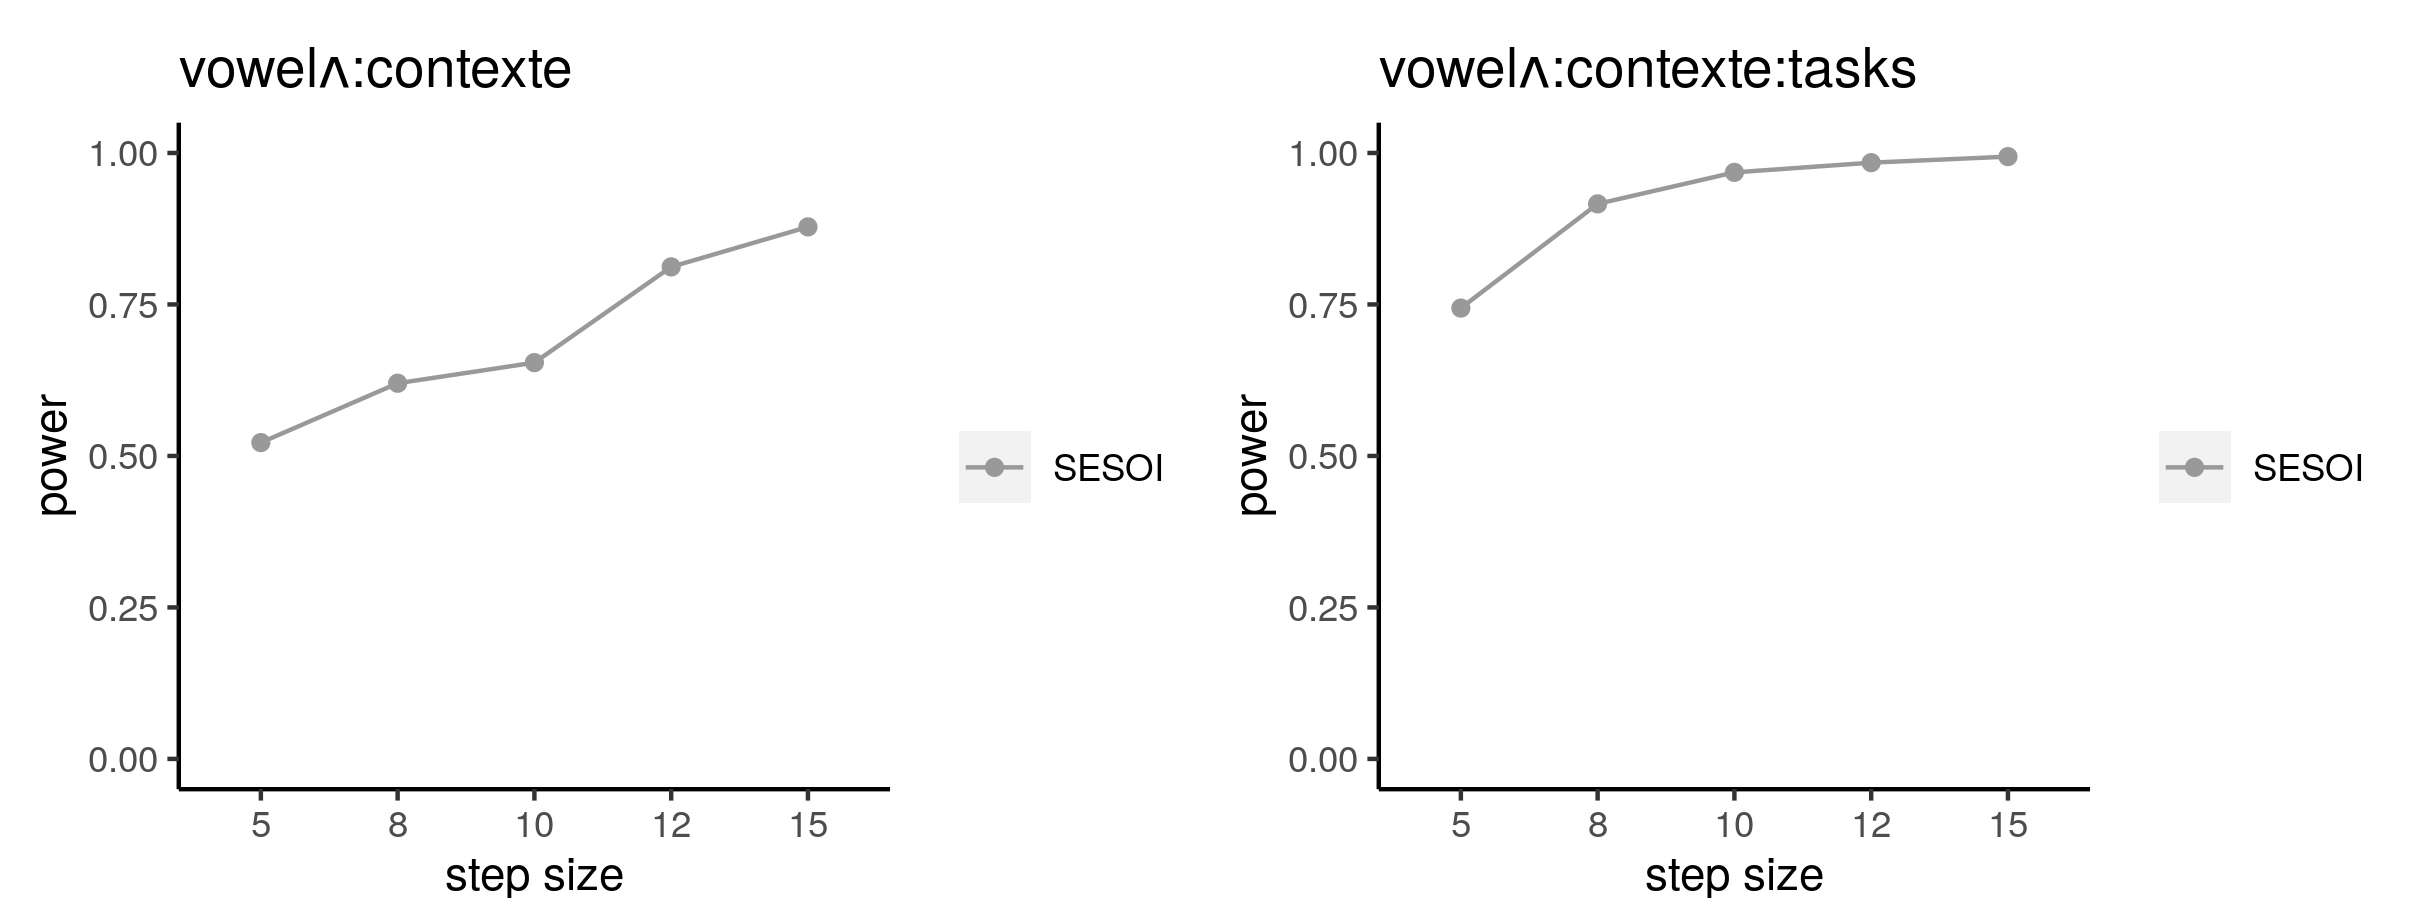
\includegraphics[width=\textwidth]{powerplot_f1_plus5} 
		\caption{Effect size = observed effect size + 5\%} \label{f1_plus5}
	\end{subfigure}
	
	
	\begin{subfigure}[t]{0.8\textwidth}
		\centering
		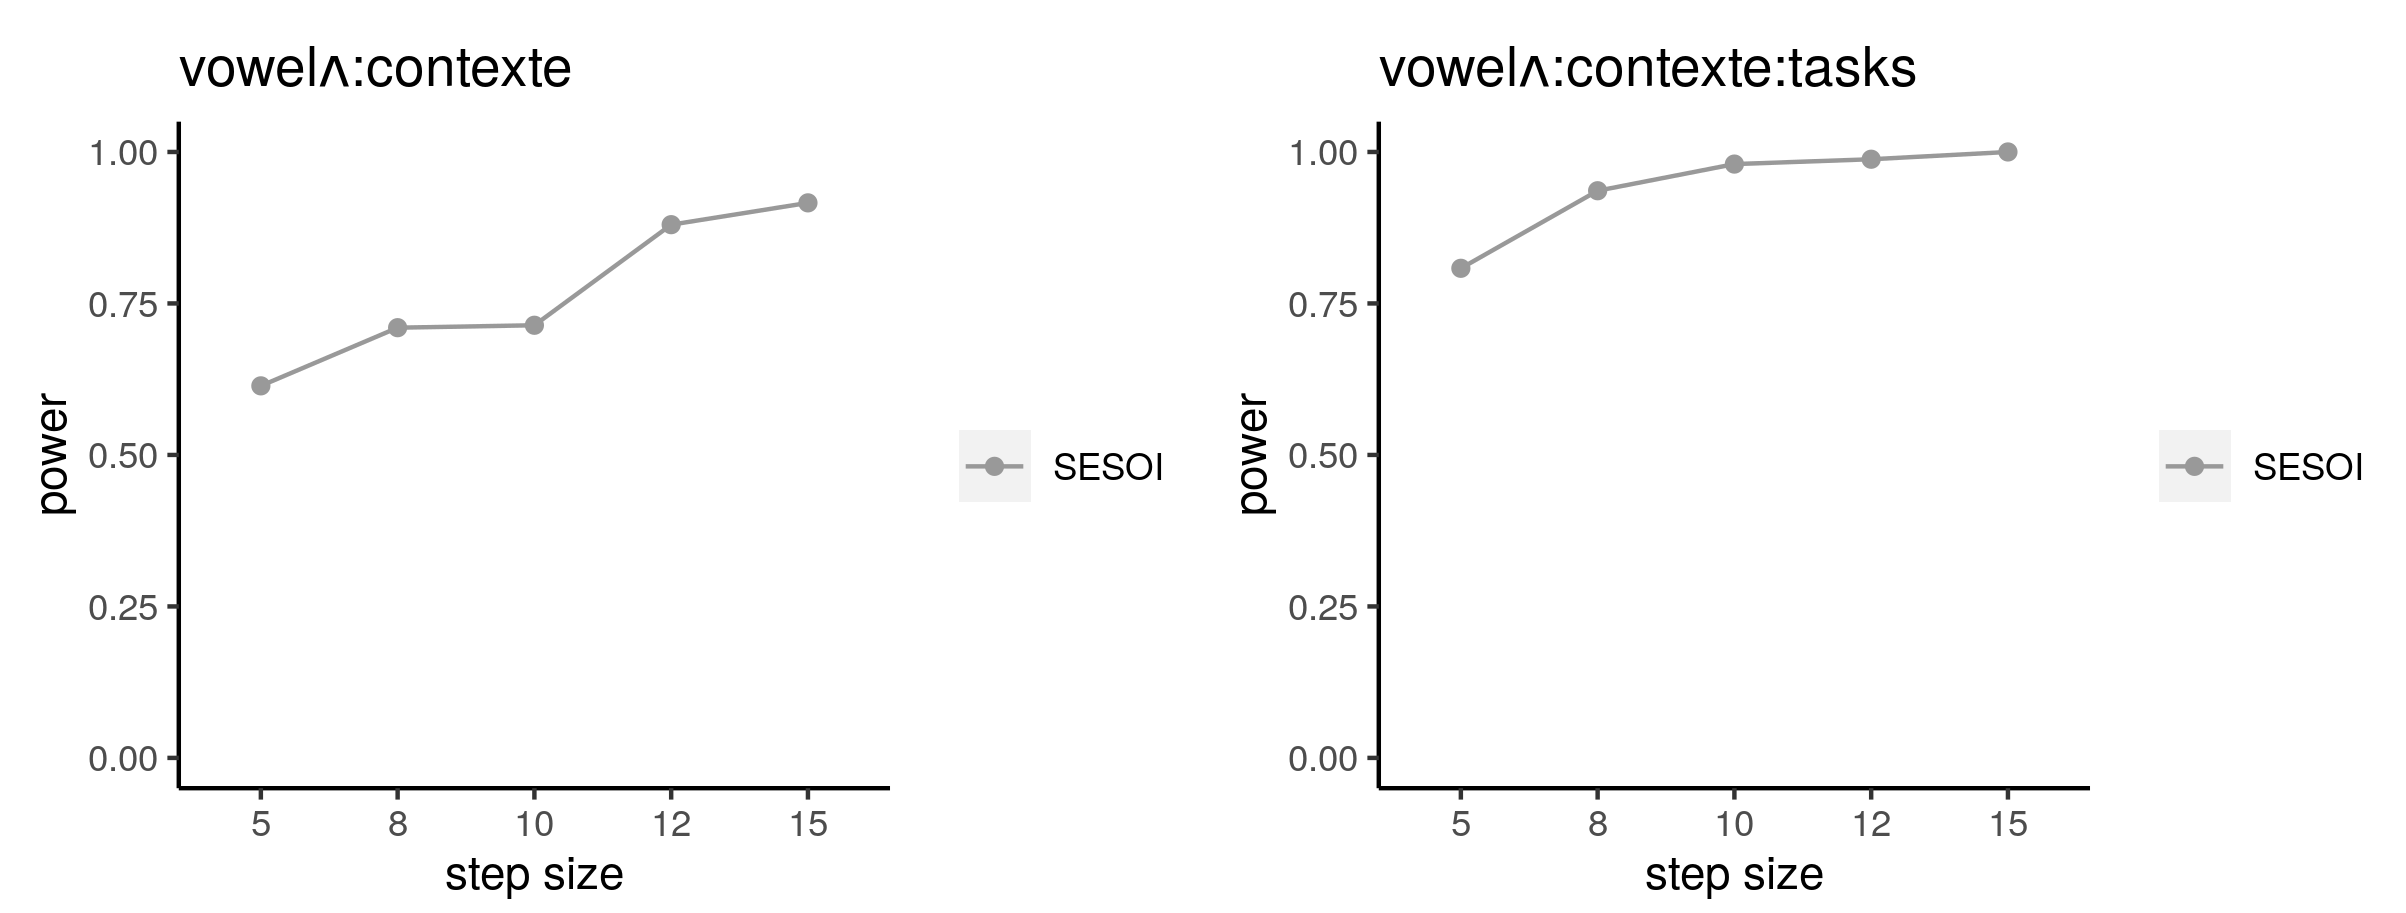
\includegraphics[width=\textwidth]{powerplot_f1_plus15} 
		\caption{Effect size = observed effect size + 15\%} \label{f1_plus15}
	\end{subfigure}
	
	\caption{Power analysis for fixed effects of interest at varying sample sizes: F1}
	
\end{figure}


\begin{figure}[!htb] \label{figure_power_analysis_f2}
	\centering
	\begin{subfigure}[t]{0.8\textwidth}
		\centering
		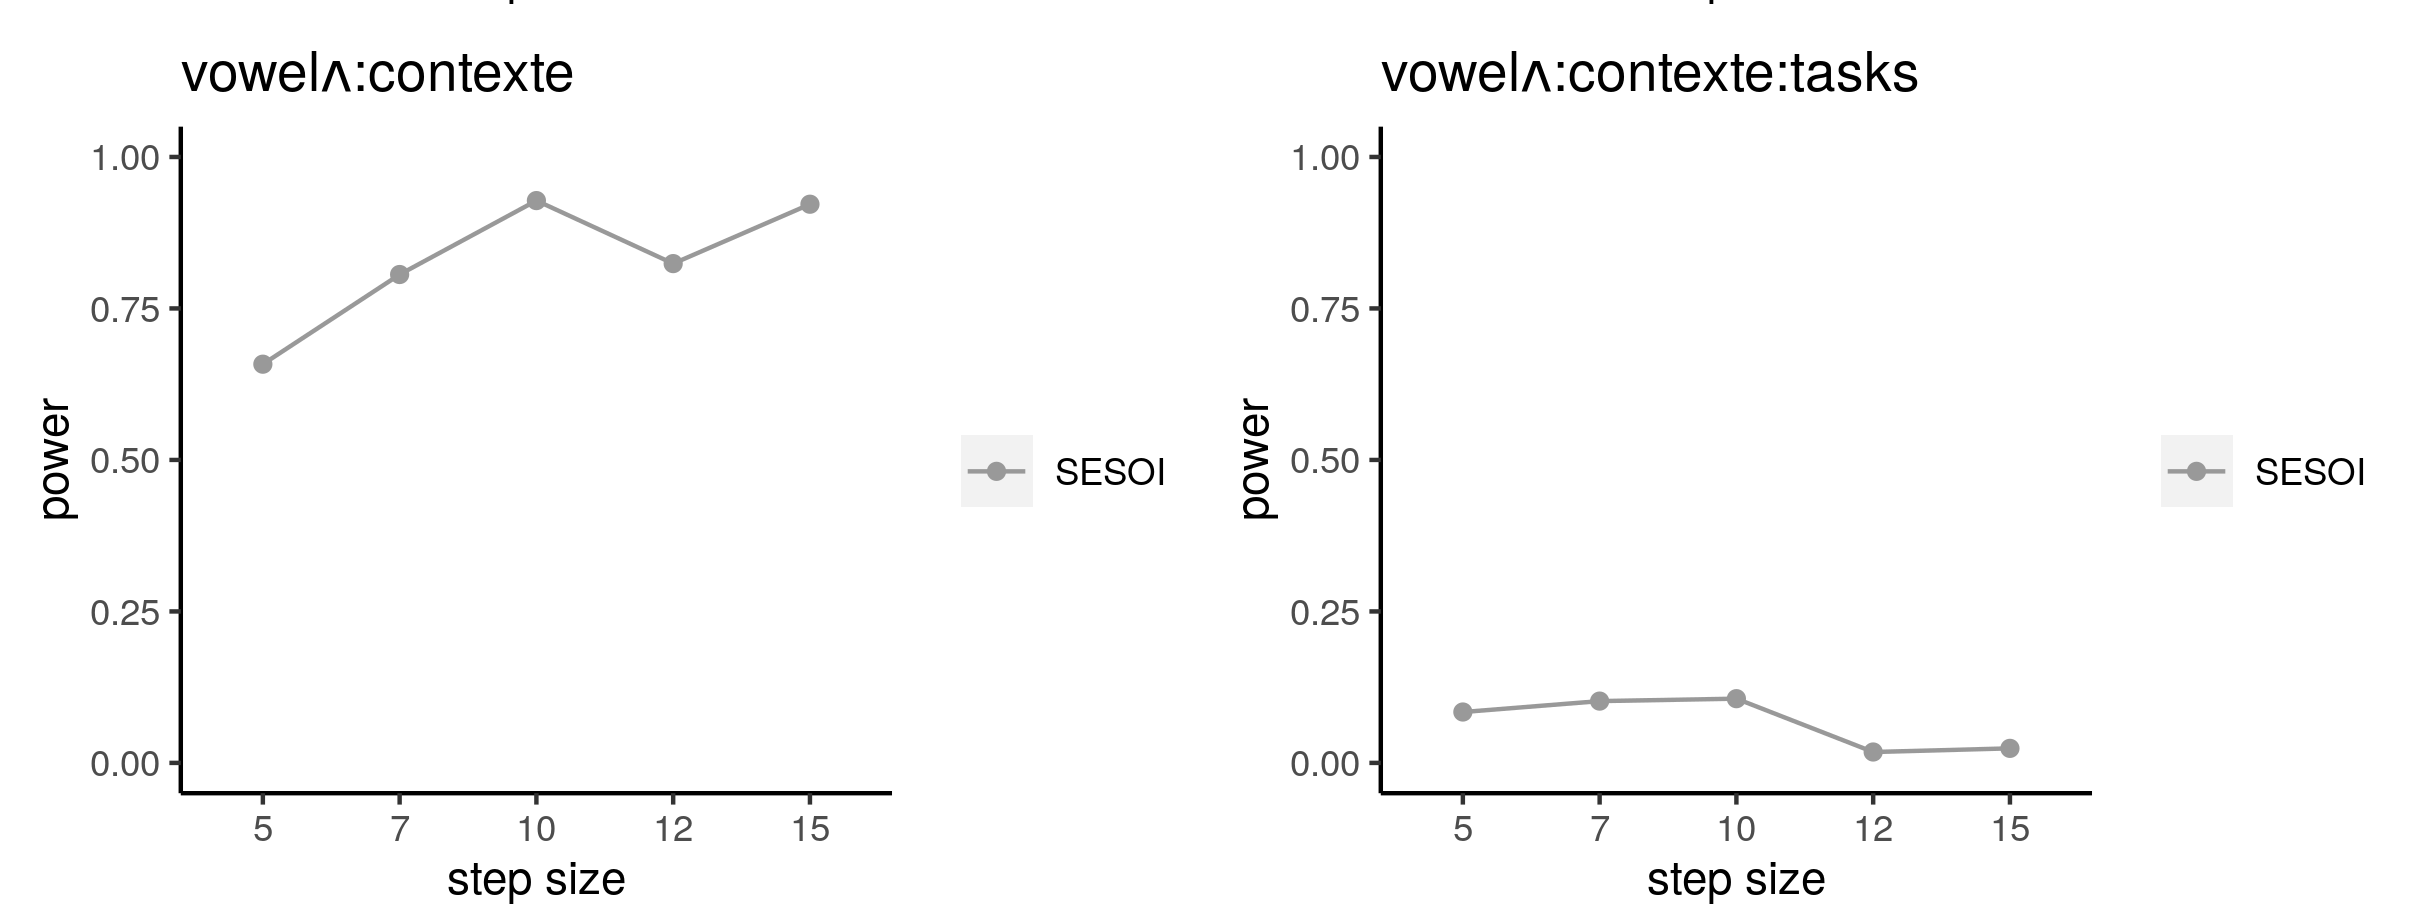
\includegraphics[width=\textwidth]{powerplot_f2_minus15} 
		\caption{Effect size = observed effect size - 15\%} \label{f2_minus15}
	\end{subfigure}
	
	\begin{subfigure}[t]{0.8\textwidth}
		\centering
		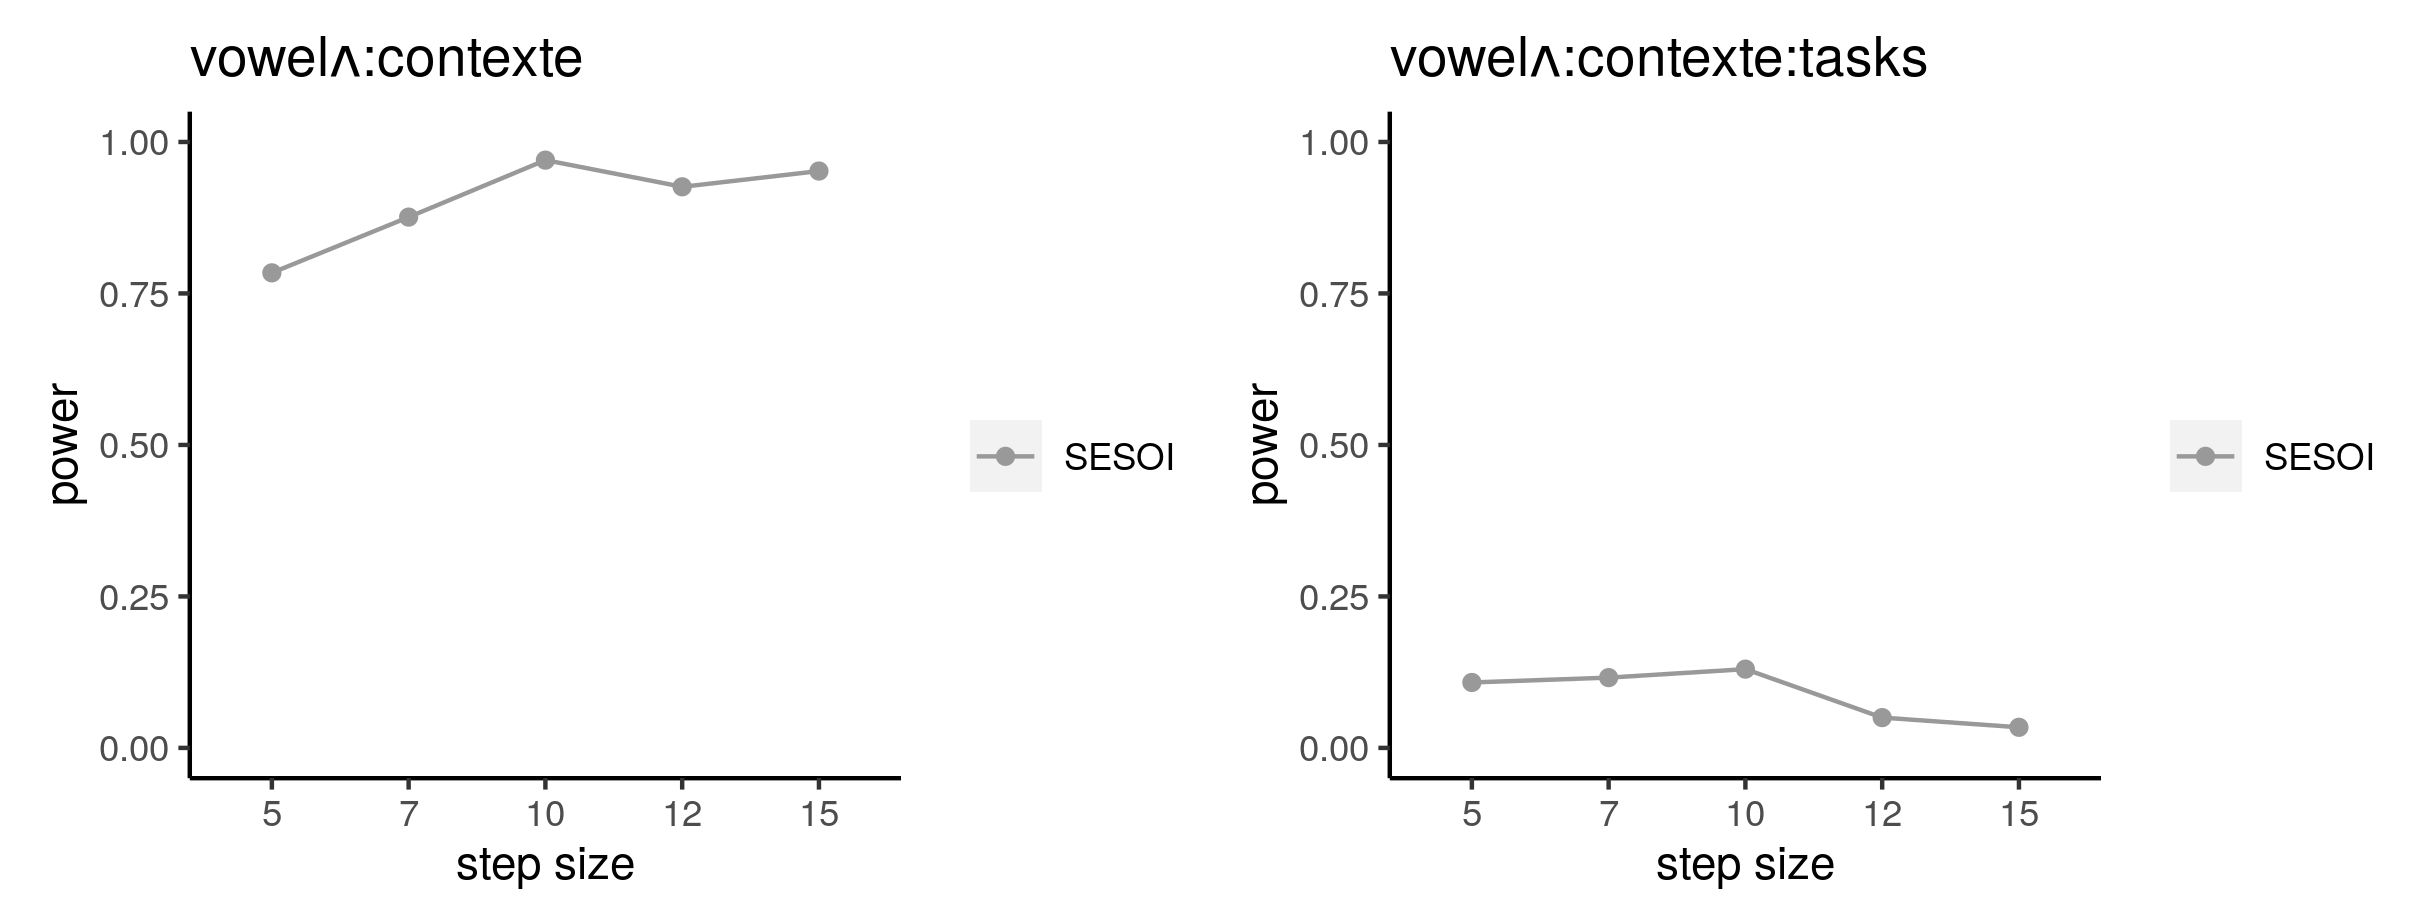
\includegraphics[width=\textwidth]{powerplot_f2_minus5} 
		\caption{Effect size = observed effect size - 5\%} \label{f2_minus5}
	\end{subfigure}
	
	
	\begin{subfigure}[t]{0.8\textwidth}
		\centering
		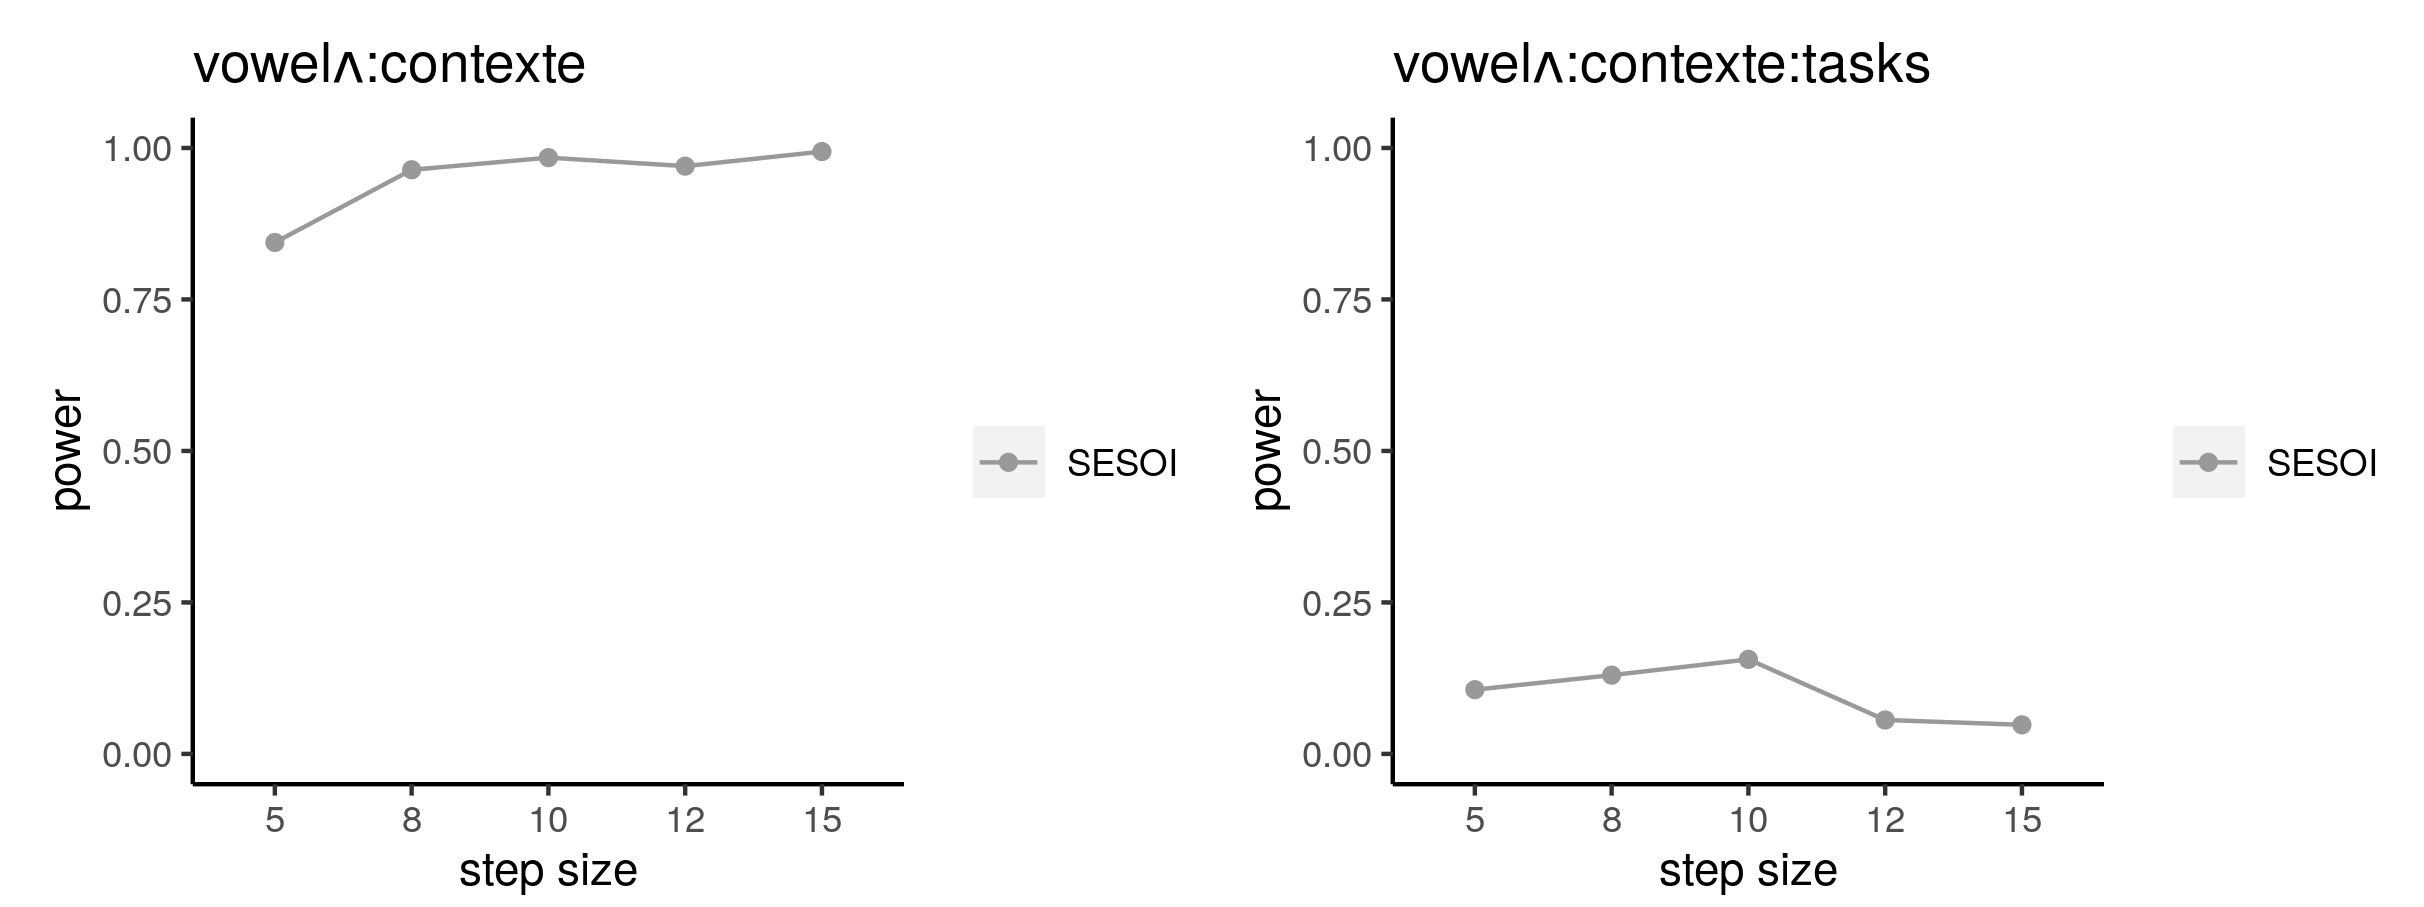
\includegraphics[width=\textwidth]{powerplot_f2_plus5} 
		\caption{Effect size = observed effect size + 5\%} \label{f2_plus5}
	\end{subfigure}
	
	
	\begin{subfigure}[t]{0.8\textwidth}
		\centering
		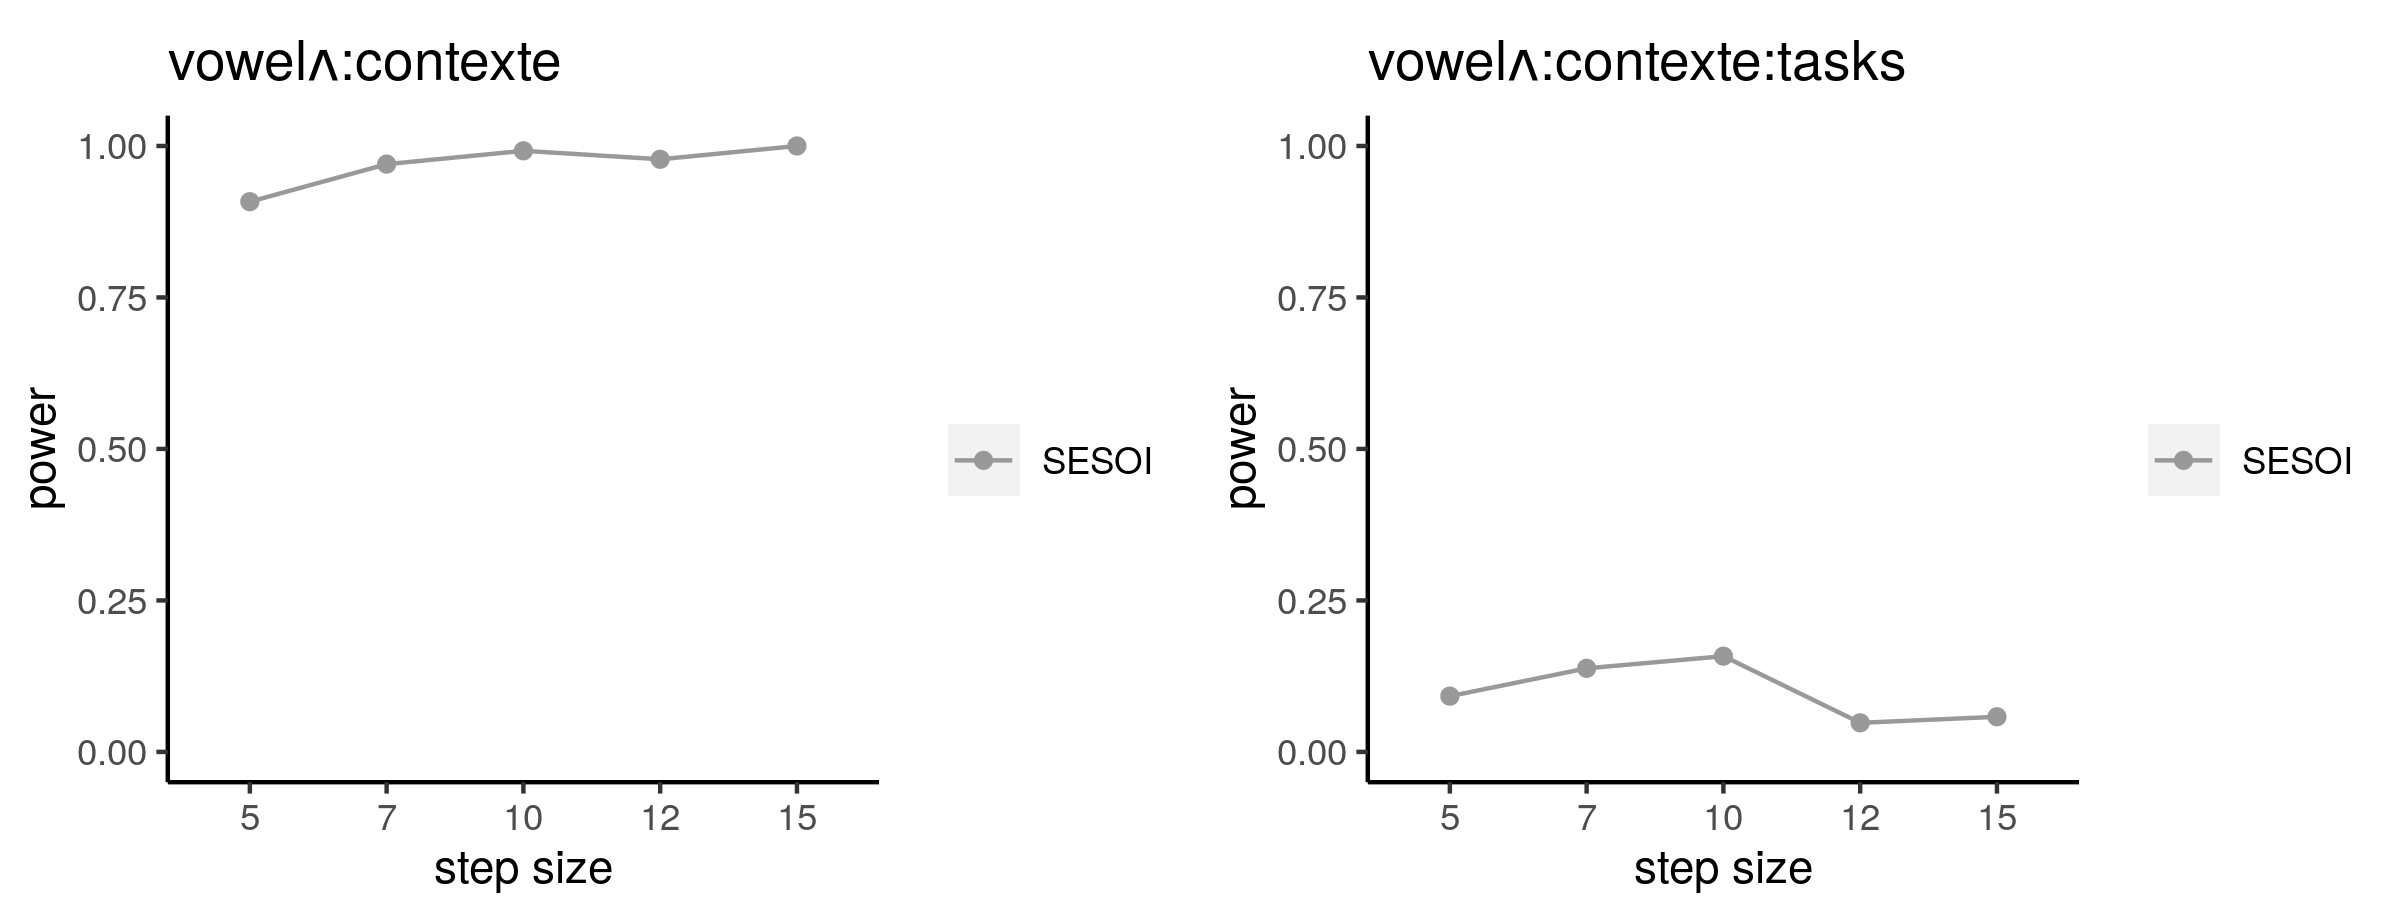
\includegraphics[width=\textwidth]{powerplot_f2_plus15} 
		\caption{Effect size = observed effect size + 15\%} \label{f2_plus15}
	\end{subfigure}
	
	\caption{Power analysis for fixed effects of interest at varying sample sizes: F2}
	
\end{figure}

\newpage



\clearpage
\bibliography{references}

\end{document}